\chapter{Implémentation}
\label{chap:implementation}


Dans les chapitres précédents, nous avons commencé par décrire
la méthode Galerkin Discontinue (GD) appliquée aux équations de Maxwell en passant
par la mise sous forme d'un système de Friedrichs.
Rappelons que cette méthode s'applique à tout système de lois
de conservation pysique.
Nous avons ensuite présenté des modèles de simulation permettant
de modéliser des matériaux spécifiques tels que les conducteurs parfaits
(métaux) et les plaques minces de diélectriques, ou de calculer
la solution des équations de Maxwell en domaine infini simulé
à l'aide de conditions limites absorbantes.
\\

Cette méthode peut théoriquement être appliquée à
tout type de maillage. Nous étudions ici le cas des maillages
composés de mailles hexaédriques à arêtes droites.
L’utilisation des hexaèdres a par exemple été étudiée par Cohen
\textit{et al.} \cite{Coh-Fer-Per-2006-1}.
Une autre possibilité est l'utilisation des mailles
tétraédriques qui a notamment été étudiée par Hesthaven \textit{et al.}
\cite{Hesthaven:2007:NDG:1557392} et Lanteri \textit{et al.}
\cite{lohrengel:hal-00210500}.
Les hexaèdres permettent diverses optimisations de la formulation GD et
sont bien adaptés à la parallélisation sur processeur graphique.

Dans ce chapitre, nous introduisons l'espace d’approximation
dans lequel nous chercherons la solution numérique de notre problème.
Cet espace est engendré par des fonctions de base à support
inclus dans une unique maille. Le choix de ces fonctions de base
est varié. Nous pouvons citer par exemple les travaux de Kopriva \textit{et al.}
\cite{Kopriva10.1002}, Lu \textit{et al.} \cite{LU2004549}, Cheong \textit{et al.}
\cite{779907} et Cohen \textit{et al.} \cite{Coh-Fer-Per-2006-1}.
%\todo{heu, je ne citerai pas brezzi ici ou alors un de ses travaux sur Maxwell, trouver d'autres refs}
Dans le cas du solveur \texttt{teta-clac} que nous avons implémenté, nous utilisons
une base de polynômes dite nodale. Cette base est constituée
de produits tensoriels de polynômes d’interpolation de Lagrange.
Les points d’interpolation choisis sont les points d’intégration de
Gauss-Legendre.

Avec l'utilisation combinée des hexaèdres,
ce choix de polynômes et de points d’interpolation
permet plusieurs optimisations (simplifications au sein des intégrales)
qui rendrent la méthode GD particulièrement efficace.
Dans le cas du solveur \texttt{schnaps} que nous évoquerons au chapitre
\ref{chap:runtimes}, les points d’intégration choisis sont ceux de
Gauss-Lobatto.

Nous finissons par décrire les schémas d'intégration en temps
actuellement les plus souvent utilisés par le solveur :
les schémas de type Runge-Kutta.
Nous donnons aussi $2$ diagnostics permettant d'étudier
la stabilité du schéma couplé espace-temps.
\\



\section{Elément de référence}
\label{sect:maille_de_reference}


Dans un premier temps, nous construisons l’espace d’approximation dans
lequel nous cherchons la solution numérique de notre problème. La construction
de cet espace s’appuie sur la définition d’un élément de référence, ici
le cube unité, noté $\HexaRef = \ItvCC{0}{1}^{3}$.
Nous notons $\xref = \NodeDef{\xref}$ un point de cet espace.
Une transformation géométrique
nous permettra de passer du cube de référence à une maille hexaédrique $\L$.

Les fonctions de base sont alors constituées de compositions entre cette
transformation et des fonctions polynomiales définies sur $\HexaRef$.
Ces fonctions polynomiales sont des produits tensoriels de polynômes de Lagrange
associés aux points d'intégration de Gauss-Legendre. Ces derniers nous serviront
également à définir des formules de quadrature permettant d’estimer les intégrales
volumiques et surfaciques apparaissant dans la méthode GD.

Ces choix de fonctions
de base et de formules de quadrature permettent diverses simplifications de
la formulation GD discrète.
\\


%  PH: N etoile
Dans la suite, nous noterons $\Deg \in \EnsN^\star$, l’ordre d’approximation du schéma.

\begin{remark}
	Dans cette section, nous ferons commencer la numérotation des indices
	à partir de l’indice 0. Ce choix permet certaines simplifications
	d’écriture et correspond aussi à la numérotation du langage C++ utilisé
	pour programmer le solveur.
	\\
\end{remark}


\subsection{Points d'intégration}
\label{ssect:points_integration}


Soient $(\GLn_p)_{p \in \RangeDeg}$ et $(\GLw_p)_{p \in \RangeDeg}$
les points et poids de quadrature
de Gauss-Legendre de degré $\Deg$ sur l’intervalle $\ItvCC{0}{1}$.
Nous allons passer de la dimension $1$ à la dimension $3$ par des techniques
de produits tensoriels. À tout multi-indice $\VMId{p}$ d’entiers compris
entre $0$ et $\Deg$ nous pouvons associer de manière bijective un unique entier
$i = \VMIdToId{p}$ compris entre $0$ et $\VNPG - 1$.
Des divisions euclidiennes permettent de retrouver le multi-indice
$\VMId{p}$ de manière unique à partir de $i$.


Nous pouvons alors définir $\VNPG$ points d’intégration volumiques :
\begin{align}
	\GLN{i} = \Node{\GLn_\MId{p}{0}}{\GLn_\MId{p}{1}}{\GLn_\MId{p}{2}}
	\in \HexaRef
\end{align}
et les $\VNPG$ poids d’intégration associés :
\begin{align}
	\GLW{i} = \GLw_\MId{p}{0} \GLw_\MId{p}{1} \GLw_\MId{p}{2}
	\in \EnsR^{\star +} .
\end{align}

Nous approcherons alors les intégrales sur $\HexaRef$ par la formule de
quadrature en dimension $3$ découlant directement de la formule de quadrature sur $\ItvCC{0}{1}$ :
\begin{align}
	\int_{\HexaRef} \psi (\xref) d\xref \approx
	\VSum{i} \GLW{i} \psi (\GLN{i})
	\label{eq:quadrature_volume} .
\end{align}
En découle aussi la propriété suivante :
\begin{proposition}
	La formule de quadrature \eqref{eq:quadrature_volume} associée aux points
	$(\GLN{i})$ et poids $(\GLW{i})$ est exacte pour des produits
	tensoriels de polynômes de degré au plus $2 \Deg + 1$.
\end{proposition}


Ajoutons à ces points d’intégration, des points d’intégration situés sur les
faces du cube $\HexaRef$. Notons $(\QuadRef_f)_{f \in \Range{0}{5}}$
les $6$ faces quadrangulaires du cube $\HexaRef$.
Nous avons choisi la numérotation suivante des faces du cube de référence :
\begin{equation}
	\begin{aligned}
		\QuadRef_0 &= \ItvCC{0}{1} \times \lbrace 0 \rbrace \times \ItvCC{0}{1} , \\
		\QuadRef_1 &= \lbrace 1 \rbrace \times \ItvCC{0}{1} \times \ItvCC{0}{1} , \\
		\QuadRef_2 &= \ItvCC{0}{1} \times \lbrace 1 \rbrace \times \ItvCC{0}{1} , \\
		\QuadRef_3 &= \lbrace 0 \rbrace \times \ItvCC{0}{1} \times \ItvCC{0}{1} , \\
		\QuadRef_4 &= \ItvCC{0}{1} \times \ItvCC{0}{1} \times \lbrace 0 \rbrace , \\
		\QuadRef_5 &= \ItvCC{0}{1} \times \ItvCC{0}{1} \times \lbrace 1 \rbrace .
	\end{aligned}
\end{equation}

Nous définissons sur la face $\QuadRef_f$, $\SNPG$ points d’intégration
surfaciques notés $(\GLN{f,i})$.
Ces points sont numérotés de $0$ à $\SNPG - 1$ sur chaque face.
Comme précédemment cette numérotation permet de retrouver facilement
les indices des points unidimensionnels à partir de divisions euclidiennes.
Ces points sont les projetés sur les faces des points d’intégration dans le
volume (figure \ref{img:hexa_ref}).

\begin{figure}[h]
	\begin{center}
		\caption{
			\label{img:hexa_ref}
			Points d’intégration volumiques (« $+$ » bleus) et surfaciques
			(« $\times$ » verts) de l’élément de référence $\HexaRef$ pour $\Deg = 2$.
			Les alignements entre ces points sont représentés par les lignes
			pointillées.
		}
		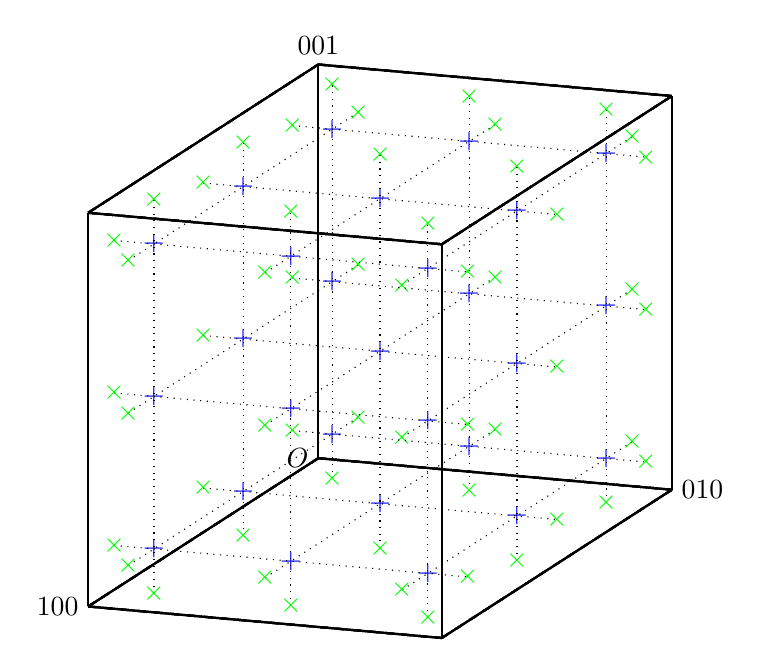
\begin{tikzpicture}[scale=5,rotate around x=270,rotate around z=258]
			% cube
			\def \c {0,1}
			\foreach \x in \c
			\foreach \y in \c
			\foreach \z in \c {
				\ifthenelse{\x = 0 \AND \y = 0 \AND \z = 0}{
					\ifthenelse{\x = 0}{\draw [dashed,thick] (0,\y,\z) -- (1,\y,\z);}{}
					\ifthenelse{\y = 0}{\draw [dashed,thick] (\x,0,\z) -- (\x,1,\z);}{}
					\ifthenelse{\z = 0}{\draw [dashed,thick] (\x,\y,0) -- (\x,\y,1);}{}
				}{
					\ifthenelse{\x = 0}{\draw [-,thick] (0,\y,\z) -- (1,\y,\z);}{}
					\ifthenelse{\y = 0}{\draw [-,thick] (\x,0,\z) -- (\x,1,\z);}{}
					\ifthenelse{\z = 0}{\draw [-,thick] (\x,\y,0) -- (\x,\y,1);}{}
				}
			}
			% annotations
			\draw (0,0,0) node[left] {$O$};
			\draw (1,0,0) node[left] {$\Node{1}{0}{0}$};
			\draw (0,1,0) node[right] {$\Node{0}{1}{0}$};
			\draw (0,0,1) node[above] {$\Node{0}{0}{1}$};
			
			% gauss legendre: 0.1127, 0.5, 0.8873
			\def \pgs {0.1127,0.5,0.8873}
			% points volumiques
			\foreach \x in \pgs
			\foreach \y in \pgs
			\foreach \z in \pgs {
				\draw (\x,\y,\z) node[blue] {$\bm{+}$};
			}
			% points surface et lignes pointilées direction x
			\foreach \y in \pgs
			\foreach \z in \pgs {
				\draw [dotted] (0,\y,\z) -- (1,\y,\z);
				\foreach \x in \c {
					\draw (\x,\y,\z) node[green] {$\bm{\times}$};
				}
			}
			% points surface et lignes pointilées direction y
			\foreach \x in \pgs
			\foreach \z in \pgs {
				\draw [dotted] (\x,0,\z) -- (\x,1,\z);
				\foreach \y in \c {
					\draw (\x,\y,\z) node[green] {$\bm{\times}$};
				}
			}
			% points surface et lignes pointilées direction z
			\foreach \x in \pgs
			\foreach \y in \pgs {
				\draw [dotted] (\x,\y,0) -- (\x,\y,1);
				\foreach \z in \c {
					\draw (\x,\y,\z) node[green] {$\bm{\times}$};
				}
			}
		\end{tikzpicture}
	\end{center}
\end{figure}


\newcommand{\FPermut}{\sigma_{\mathrm{ori}}} % Permutation des faces

Afin de les définir rigoureusement, nous commençons par considérer
le tableau suivant, donnant pour chaque face les directions des deux axes
tangents à la face puis de l’axe normal à la face. La dernière colonne du
tableau correspond à la valeur sur la face de la dernière coordonnée :
\begin{align}
	\FPermut =
	\begin{pmatrix}
		0 & 2 & 1 & 0 \\
		1 & 2 & 0 & 1 \\
		2 & 0 & 1 & 1 \\
		2 & 1 & 0 & 0 \\
		1 & 0 & 2 & 0 \\
		0 & 1 & 2 & 1
	\end{pmatrix} .
\end{align}
Par exemple, pour la face $0$ (\textit{i.e.} la première ligne du tableau),
les axes tangents correspondent à ceux des composantes $0$ et $2$,
la direction normale correspond à l'axe de la composante $1$
et la coordonnée sur cet axe normal est $\xref_1 = 0$.

Considérons maintenant l'indice $i$ compris entre $0$ et $\SNPG - 1$
d’un point de face. Nous pouvons trouver de façon unique deux indices
$\MId{p}{0}$ et $\MId{p}{1}$ compris entre $0$ et $\Deg$ tels que $i = \SMIdToId{p}$.
Alors le point correspondant sur la face $f$ est donné par :
\begin{align}
	\GLN{f,i} = \Node{\alpha_0}{\alpha_1}{\alpha_2}
\end{align}
avec
\begin{align}
	\alpha_{\FPermut(f,0)} = \GLn_\MId{p}{0} , \quad
	\alpha_{\FPermut(f,1)} = \GLn_\MId{p}{1} , \quad
	\alpha_{\FPermut(f,2)} = \FPermut(f,3) .
\end{align}
À ce point d’intégration correspond le poids d’intégration suivant :
\begin{align}
	\GLW{f,i} = \GLw_\MId{p}{0} \GLw_\MId{p}{1} .
\end{align}

Ces points et poids d’intégration définissent une formule de quadrature permettant
d’approcher les intégrales sur les faces de l’élément $\HexaRef$ :
\begin{align}
	\int_{\QuadRef_f} \psi (\xref) d\xref \approx
	\SSum{i} \GLW{f,i} \psi (\GLN{f,i})
	\label{eq:quadrature_surface} .
\end{align}

Grâce aux propriétés de quadrature de Gauss-Legendre, nous avons la propriété
suivante :
\begin{proposition}
	La formule de quadrature \eqref{eq:quadrature_surface} associée aux points
	$(\GLN{f,i})$ et poids $(\GLW{f,i})$ est exacte pour des produits
	tensoriels de polynômes de degrés au plus $2 \Deg + 1$.
\end{proposition}

Nous pouvons encore définir le projeté sur la face $\QuadRef_f$
d’un point d’intégration volumique $\GLN{i}$, avec
$i = \VMIdToId{p}$.
Cette projection nous permettra d'exprimer des simplifications qui appraîtront
lors de l'extrapolation des champs sur les faces.
Il s'agit du point $\GLN{f,j}$ dont l'indice
$j$ peut être calculé à l'aide de l’application $\pi$ définie telle que :
\begin{equation}
	\begin{aligned}
		j &= \pi (f,i) \\
		&= \pi (f,\VMIdToId{p}) \\
		&= \MId{p}{\FPermut(f,0)} + (\Deg + 1) \MId{p}{\FPermut(f,1)} .
	\end{aligned}
\end{equation}
%  PH: pb: il n'y a pas i ni i' dans la formule

Enfin, nous munissons les faces de l’élément de référence d’une normale
unitaire sortante notée $\hat{\n}$ (figure \ref{img:hexa_ref_normales}) :
\begin{equation}
	\hat{\n} =
	\begin{cases}
		\Vect{0}{-1}{0} & \text{sur la face 0,} \\
		\Vect{1}{0}{0} & \text{sur la face 1,} \\
		\Vect{0}{1}{0} & \text{sur la face 2,} \\
		\Vect{-1}{0}{0} & \text{sur la face 3,} \\
		\Vect{0}{0}{-1} & \text{sur la face 4,} \\
		\Vect{0}{0}{1} & \text{sur la face 5.}
	\end{cases}
\end{equation}


\begin{figure}[h]
	\begin{center}
		\caption{
			\label{img:hexa_ref_normales}
			Orientation des normales des faces de l’élément de référence.
			La normale à la face $\QuadRef_f$ est notée $\hat{\n}_f$.
		}
		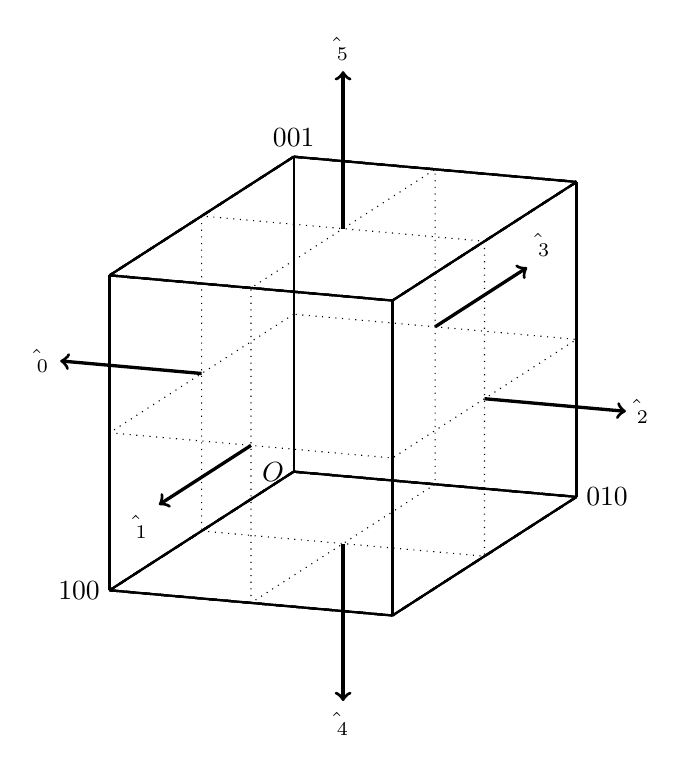
\begin{tikzpicture}[scale=4,rotate around x=270,rotate around z=258]
			% cube
			\def \c {0,1}
			\foreach \x in \c
			\foreach \y in \c
			\foreach \z in \c {
				\ifthenelse{\x = 0 \AND \y = 0 \AND \z = 0}{
					\ifthenelse{\x = 0}{\draw [dashed,thick] (0,\y,\z) -- (1,\y,\z);}{}
					\ifthenelse{\y = 0}{\draw [dashed,thick] (\x,0,\z) -- (\x,1,\z);}{}
					\ifthenelse{\z = 0}{\draw [dashed,thick] (\x,\y,0) -- (\x,\y,1);}{}
				}{
					\ifthenelse{\x = 0}{\draw [-,thick] (0,\y,\z) -- (1,\y,\z);}{}
					\ifthenelse{\y = 0}{\draw [-,thick] (\x,0,\z) -- (\x,1,\z);}{}
					\ifthenelse{\z = 0}{\draw [-,thick] (\x,\y,0) -- (\x,\y,1);}{}
				}
			}
			% annotations
			\draw (0,0,0) node[left] {$O$};
			\draw (1,0,0) node[left] {$\Node{1}{0}{0}$};
			\draw (0,1,0) node[right] {$\Node{0}{1}{0}$};
			\draw (0,0,1) node[above] {$\Node{0}{0}{1}$};
			
			% lignes pointilées sur faces
			\draw [dotted] (0.5,0,0) -- (0.5,1,0) -- (0.5,1,1) -- (0.5,0,1) -- cycle;
			\draw [dotted] (0,0.5,0) -- (1,0.5,0) -- (1,0.5,1) -- (0,0.5,1) -- cycle;
			\draw [dotted] (0,0,0.5) -- (1,0,0.5) -- (1,1,0.5) -- (0,1,0.5) -- cycle;
			
			% normales
			\draw [->,very thick] (0.5,0,0.5) -- (0.5,-0.5,0.5) node[left] {$\hat{\n}_0$};
			\draw [->,very thick] (1,0.5,0.5) -- (1.5,0.5,0.5) node[below left] {$\hat{\n}_1$};
			\draw [->,very thick] (0.5,1,0.5) -- (0.5,1.5,0.5) node[right] {$\hat{\n}_2$};
			\draw [->,very thick] (0,0.5,0.5) -- (-0.5,0.5,0.5) node[above right] {$\hat{\n}_3$};
			\draw [->,very thick] (0.5,0.5,0) -- (0.5,0.5,-0.5) node[below] {$\hat{\n}_4$};
			\draw [->,very thick] (0.5,0.5,1) -- (0.5,0.5,1.5) node[above] {$\hat{\n}_5$};
		\end{tikzpicture}
	\end{center}
\end{figure}


Après avoir défini l'espace de référence, nous allons le munir d'une base de fonctions
qui vont nous permettre d'exprimer la solution et de la stocker sous forme discrète.
\\


\subsection{Fonctions de base}
\label{ssect:fonctions_de_base}

Considérons maintenant les polynômes de Lagrange $(l_p)_{p \in \RangeDeg}$
associés aux points $(\GLn_p)_{p \in \RangeDeg}$.
Ces polynômes sont donnés par :
\begin{align}
	l_p(\GLn) = \prod_{\substack{q=0 \\ q \ne p}}^{\Deg}
	\frac{\GLn - \GLn_q}{\GLn_p - \GLn_q}
\end{align}
et vérifient :
\begin{align}
	l_p(\GLn_q) = \delta_{p,q}
\end{align}
où $\delta_{p,q}$ est le symbole de Kronecker qui vaut $1$ si $p = q$
et $0$ sinon.


Nous définissons la base d’approximation sur $\HexaRef$ comme étant formée des
produits tensoriels des polynômes $(l_p)$. Plus précisément, ces fonctions
de base sont données par :
\begin{equation}
	\begin{aligned}
		\PsiRef{i} : \HexaRef &\to \EnsR \\
		\xref &\mapsto
		l_\MId{p}{0}(\xref_0)
		l_\MId{p}{1}(\xref_1)
		l_\MId{p}{2}(\xref_2)
	\end{aligned}
\end{equation}
où $i = \VMIdToId{p}$.

\begin{proposition}
	La formule de quadrature \eqref{eq:quadrature_volume} est exacte pour des
	combinaisons linéaires de produits de fonctions de base décrites plus haut.
	De plus,
	\begin{align}
		\int_{\HexaRef} \VSum{i} \VSum{j}
		a_{i,j} \PsiRef{i} \PsiRef{j} d\xref =
		\VSum{i} a_{i,i} \GLW{i} .
	\end{align}
\end{proposition}

\begin{remark}
	La formule de quadrature \eqref{eq:quadrature_volume} est exacte, car nous
	utilisons des points de Gauss-Legendre. Si nous utilisions des points de
	Gauss-Lobatto, la proposition précédente ne serait plus vraie.
\end{remark}

%  PH: dire combien de calculs ça fait gagner
La proposition suivante nous permet de simplifier l’extrapolation des
champs sur les points d’intégration surfaciques. Elle nous donne
le sous-ensemble des $\Deg + 1$ fonctions de base nécessaire à
l'extrapolation des champs sur un point de face donné.
Sans cette simplification, l’extrapolation des champs nécessiterait
d'utiliser les $\VNPG$ fonctions de base de la maille pour chaque
point d’intégration surfacique.

\begin{proposition} \label{prop:projection_face}
	Une fonction de base donnée est nulle en tous points d’intégration
	surfaciques d'une face, excepté celui correspondant au projeté du point
	volumique correspondant à cette fonction de base. Autrement dit,
	\begin{equation}
		\PsiRef{i}(\GLN{f,j}) =
		\begin{cases}
			l_\MId{p}{\FPermut(f,2)}(\FPermut(f,3)) & \mathrm{si} \; j = \pi(f,i) , \\
			0 & \mathrm{sinon} .
		\end{cases}
	\end{equation}
\end{proposition}

\begin{proof}
	Soit $\PsiRef{i}$ une fonction de base et $\GLN{i}
	= \Node{\GLn_\MId{p}{0}}{\GLn_\MId{p}{1}}{\GLn_\MId{p}{2}}$ le point
	d'interpolation correspondant.
	Soit $\GLN{f,j}$ un point d’intégration sur la face $f$ avec
	$j = \SMIdToId{q}$.
	Alors, en ce point la fonction de base vaut :
	\begin{equation}
		\begin{aligned}
			\PsiRef{i}(\GLN{f,j}) &=
			l_\MId{p}{\FPermut(f,0)}(\GLn_\MId{q}{0})
			l_\MId{p}{\FPermut(f,1)}(\GLn_\MId{q}{1})
			l_\MId{p}{\FPermut(f,2)}(\FPermut(f,3)) \\
			&= \delta_{\MId{p}{\FPermut(f,0)},\MId{q}{0}}
			\delta_{\MId{p}{\FPermut(f,1)},\MId{q}{1}}
			l_\MId{p}{\FPermut(f,2)}(\FPermut(f,3)) \\
			&= \delta_{\pi(f,i),j}
			l_\MId{p}{\FPermut(f,2)}(\FPermut(f,3)) .
		\end{aligned}
	\end{equation}
\end{proof}


Nous allons maintenant définir la transformation géométrique
qui nous permettra de passer de la base d'approximation de référence
que nous venons de définir aux mailles physiques présentes dans le maillage étudié.
\\


\subsection{Transformation géométrique}
\label{ssect:transformation_geometrique}


Soit $(\hat{S}_i)_{i \in \Range{0}{7}}$ les huit sommets du cube unité
$\HexaRef$ donnés par :
\begin{equation}
	\begin{aligned}
		\hat{S}_0 &= \Node{0}{0}{0} , \qquad
		\hat{S}_1 = \Node{1}{0}{0} , \\
		\hat{S}_2 &= \Node{0}{1}{0} , \qquad
		\hat{S}_3 = \Node{1}{1}{0} , \\
		\hat{S}_4 &= \Node{0}{0}{1} , \qquad
		\hat{S}_5 = \Node{1}{0}{1} , \\
		\hat{S}_6 &= \Node{0}{1}{1} , \qquad
		\hat{S}_7 = \Node{1}{1}{1} .
	\end{aligned}
\end{equation}
Nous définissons les huit fonctions de forme associées à chacun de ces sommets :
\begin{equation}
	\begin{aligned}
		\phi_0(\xref) &=
		(1 - \xref_0)(1 - \xref_1)(1 - \xref_2) , \\
		\phi_1(\xref) &=
		\xref_0(1 - \xref_1)(1 - \xref_2) , \\
		\phi_2(\xref) &=
		(1 - \xref_0)\xref_1(1 - \xref_2) , \\
		\phi_3(\xref) &=
		\xref_0\xref_1(1 - \xref_2) , \\
		\phi_4(\xref) &=
		(1 - \xref_0)(1 - \xref_1)\xref_2 , \\
		\phi_5(\xref) &=
		\xref_0(1 - \xref_1)\xref_2 , \\
		\phi_6(\xref) &=
		(1 - \xref_0)\xref_1\xref_2 , \\
		\phi_7(\xref) &=
		\xref_0\xref_1\xref_2 .
	\end{aligned}
\end{equation}
Chacune des ces fonctions de forme prend une valeur nulle sur chacun des
sommets du cube unité excepté au point lui correspondant, \textit{i.e.} :
\begin{align}
	\phi_i(\hat{S}_j) = \delta_{i,j} .
\end{align}

Soit $\L$ un hexaèdre appartenant au maillage $\Mesh$. Cet hexaèdre est défini
par ses huit sommets $(S_i)_{i \in \Range{0}{7}}$. Nous appellerons
point physique et noterons $\x$ un point situé dans la maille $\L$ et nous
appellerons point de référence et noterons $\xref$ un point de $\HexaRef$.


Nous définissons alors la transformation géométrique $\TGeo{\L}$ telle que
l’image du cube unité est l’hexaèdre s’appuyant sur les huit sommets
$(S_i)_{i \in \Range{0}{7}}$. Cette transformation est donnée par
la formule classique, faisant intervenir les fonctions de forme :
\begin{align}
	\TGeo{\L}(\xref) = \sum_{i=0}^{7} \phi_i(\xref) S_i .
\end{align}
Nous supposerons que cette transformation est une bijection entre $\HexaRef$
et $\L$, et que son jacobien
\begin{align}
	\Jac{\TGeo{\L}} = \Det{\TGeo{\L}'}
\end{align}
est strictement positif en tout point de $\HexaRef$.

\begin{remark}
	Contrairement aux maillages en tétraèdres, il peut arriver qu'un mailleur
	produise exceptionnellement des hexaèdres dégénérés, c’est-à-dire que
	le jacobien de $\TGeo{\L}$ s’annule ou change de signe en certains points de $\L$.
	Il est important de vérifier, avant de lancer un calcul, que le maillage
	ne présente pas de maille dégénérée. Pour cela, nous pouvons calculer
	le jacobien $\Jac{\TGeo{\L}}$ aux points d’intégration
	et vérifier qu’il ne s’annule pas.
	C'est pourquoi, nous supposerons dans la suite que toutes les mailles
	considérées ne sont pas dégénérées et que la numérotation de leurs sommets
	garantit la positivité du jacobien des transformations associées.
\end{remark}

La transformation $\TGeo{\L}$ permet de passer explicitement de l'élément
de référence $\HexaRef$ à la maille physique $\L$. L’inverse de $\TGeo{\L}$
n’est en général pas calculable explicitement. Cependant, nous n’aurons à calculer
l’antécédent d’un point physique par cette transformation que dans certains cas
particuliers. Pour cela, nous utiliserons la méthode de Newton.

Nous définissons alors sur $\L$ une base d’approximation composée des fonctions
$(\PsiPhy{\L}{i})_{i \in \Range{0}{\VNPG - 1}}$. Ces fonctions sont
transportées sur la maille physique à partir des fonctions de base définies sur
l’élément de référence :
\begin{align}
	\forall \xref \in \HexaRef, \;
	\PsiPhy{\L}{i} \circ \TGeo{\L}(\xref) =
	\PsiRef{i}(\xref) ,
\end{align}
soit encore,
\begin{align}
	\forall \x \in \L, \;
	\PsiPhy{\L}{i}(\x) =
	\PsiRef{i} \circ \Inv{\TGeo{\L}}(\x) .
\end{align}

En général, les fonctions de base ainsi définies ne sont pas polynomiales
dans l’espace physique. Cependant, les approximations des intégrales restent
valables pour des maillages non dégénérés. Par ailleurs, nous prolongeons par
$0$ ces fonctions en dehors de la maille $\L$ :
\begin{align}
	\forall \x \notin \L, \; \PsiPhy{\L}{i}(\x) = 0 .
\end{align}

Rappelons que puisque nous utilisons une interpolation nodale, à chaque instant $t$,
l’approximation $\W$ est identifiée par ses valeurs sur les points d’intégration
des mailles $\L$. Notons $\W_i$ les composantes vectorielles de $\W$ dans
la base d’approximation relative à $\L$. $\W$ s’exprime en un point d’intégration
$\GLNPhy{\L}{i} = \TGeo{\L}(\GLN{i})$ de $\L$ par :
\begin{equation}
	\begin{aligned}
		\W(\GLNPhy{\L}{i},t) &= \VSum{j}
			\W_j(t) \PsiPhy{\L}{j}(\GLNPhy{\L}{i}) \\
		&= \VSum{j} \W_j(t) \PsiRef{j}(\GLN{i}) \\
		&= \W_i(t) .
	\end{aligned}
\end{equation}
Ainsi, la solution est entièrement définie par ses valeurs aux points d’intégration
volumiques. Nous stockerons donc en mémoire ces valeurs.

%  PH: préciser que l'intégration numérique devient approximative sinon
\begin{remark}
	Les formules de quadrature volumique \eqref{eq:quadrature_volume}
	et surfacique \eqref{eq:quadrature_surface} restent exactes sur la maille physique si
	la transformation géométrique $\TGeo{\L}$ est affine.
	Dans le cas contraire,
	l'intégration numérique devient approximative.
\end{remark}
	
\begin{remark}
	Bien que les formules de quadrature soient approximatives
	lorsque la transformation géométrique est quelconque,
	l'intégration par parties \eqref{eq:formule_de_green} utilisée
	pour obtenir la formulation GD reste exacte : l'erreur commise
	est de l'ordre de $10^{-14}$ à l'ordre d'interpolation $\Deg = 2$.
	Les erreurs commises et la maille tordue testée sont présentées
	dans la figure \ref{img:erreur_ipp}.
\end{remark}
%\todo{PH: question: même si l'intégration est inexacte, la formule d'intégration par parties reste-t-elle exacte ?}


\begin{figure}[!h]
	\begin{center}
		\caption{
			\label{img:erreur_ipp}
			Erreur commise au cours de l'intégration par parties discrète
			sur un hexaèdre quelconque (non affine).
		}
		
		\subfloat[Erreurs.]{
			\label{img:erreur_ipp_err}
			\begin{tabular}{|c|c|}
				\hline
				$\Deg$ & Erreur $\mathrm{L}^2$ \\ \hline\hline
				$0$ & $4.23 \cdot 10^{-16}$ \\	\hline
				$1$ & $4.75 \cdot 10^{-15}$ \\	\hline
				$2$ & $1.52 \cdot 10^{-14}$ \\	\hline
				$3$ & $6.63 \cdot 10^{-14}$ \\	\hline
				$4$ & $1.04 \cdot 10^{-13}$ \\	\hline
			\end{tabular}
		}
		\\
		\subfloat[Hexaèdre.]{
			\label{img:erreur_ipp_hexa}
			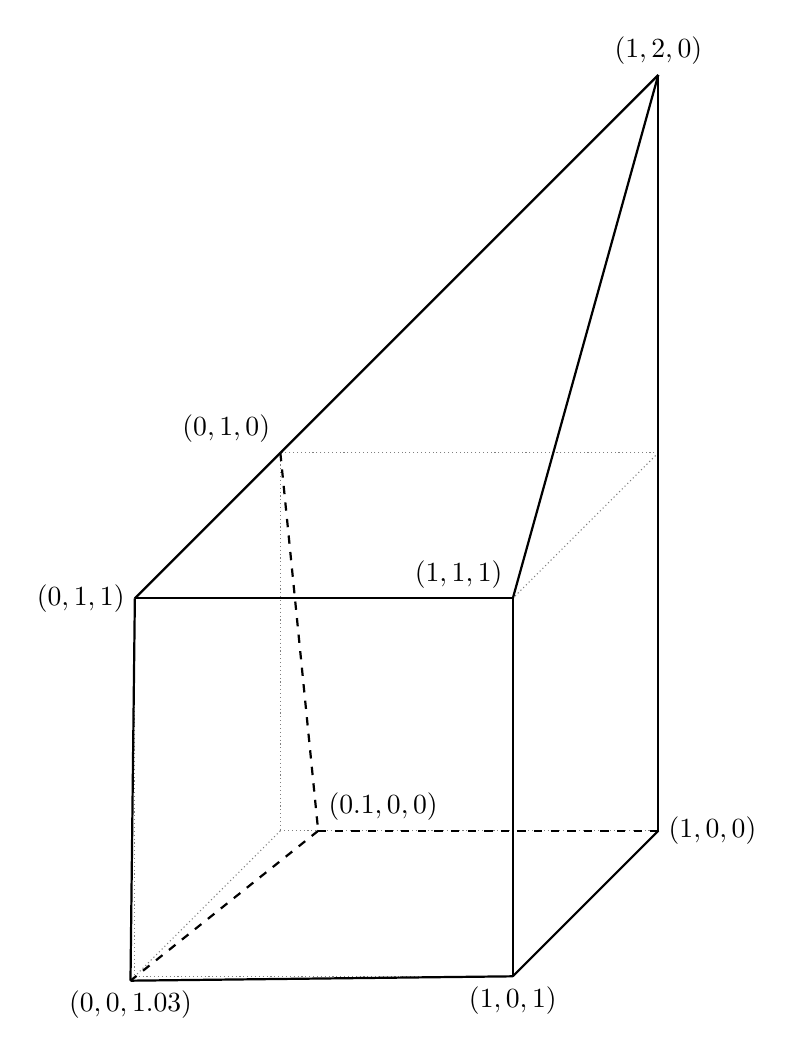
\begin{tikzpicture}[scale=4.8]
			\draw[densely dotted,gray] (0,0,0) -- (1,0,0);
			\draw[densely dotted,gray] (1,0,0) -- (1,1,0);
			\draw[densely dotted,gray] (1,1,0) -- (0,1,0);
			\draw[densely dotted,gray] (0,1,0) -- (0,0,0);
			\draw[densely dotted,gray] (0,0,1) -- (1,0,1);
			\draw[densely dotted,gray] (1,0,1) -- (1,1,1);
			\draw[densely dotted,gray] (1,1,1) -- (0,1,1);
			\draw[densely dotted,gray] (0,1,1) -- (0,0,1);
			\draw[densely dotted,gray] (0,0,0) -- (0,0,1);
			\draw[densely dotted,gray] (1,0,0) -- (1,0,1);
			\draw[densely dotted,gray] (1,1,0) -- (1,1,1);
			\draw[densely dotted,gray] (0,1,0) -- (0,1,1);

			\draw[thick,dashed] (0.1,0,0) -- (1,0,0) node[right]{$(1,0,0)$};
			\draw[thick] (1,0,0) -- (1,2,0) node[above]{$(1,2,0)$};
			\draw[thick] (1,2,0) -- (0,1,0) node[above left]{$(0,1,0)$};
			\draw[thick,dashed] (0,1,0) -- (0.1,0,0) node[above right]{$(0.1,0,0)$};
			\draw[thick] (0,0,1.03) -- (1,0,1) node[below]{$(1,0,1)$};
			\draw[thick] (1,0,1) -- (1,1,1) node[above left]{$(1,1,1)$};
			\draw[thick] (1,1,1) -- (0,1,1) node[left]{$(0,1,1)$};
			\draw[thick] (0,1,1) -- (0,0,1.03) node[below]{$(0,0,1.03)$};
			\draw[thick,dashed] (0.1,0,0) -- (0,0,1.03);
			\draw[thick] (1,0,0) -- (1,0,1);
			\draw[thick] (1,2,0) -- (1,1,1);
			\draw[thick] (0,1,0) -- (0,1,1);
			\end{tikzpicture}
		}
	\end{center}
\end{figure}


Nous allons maintenant décrire la formulation discrète obtenue en utilisant
l’espace d’approximation que nous venons de construire. Plus précisément, nous
examinerons les approximations des intégrales présentes dans la formulation
GD \eqref{eq:formulation_gd_finale} obtenues en appliquant les formules
de quadrature volumique \eqref{eq:quadrature_volume} et surfacique
\eqref{eq:quadrature_surface}.
\\


\section{Approximation des intégrales}
\label{sect:approximation_des_integrales}

En partant d’une formulation faible de notre problème de départ, nous avons
établi une formulation semi-discrète. Nous allons maintenant détailler
le calcul des différentes intégrales apparaissant dans
la formulation semi-discrète \eqref{eq:formulation_semi-discrete} lorsque
nous discrétisons la solution dans l’espace d’approximation décrit dans
la section précédente.

Pour cela, nous estimerons ces intégrales au moyen des formules de quadrature
volumique \eqref{eq:quadrature_volume} et surfacique \eqref{eq:quadrature_surface}.
Nous verrons alors diverses simplifications de ces estimations
introduites par Cohen \textit{et al.} \cite{Coh-Fer-Per-2006-1}.
\\

Notons les décompositions des champs $\W$ et $\Ptl{t}\W$ dans la base
d’approximation :
\begin{subequations}
	\begin{align}
		\W(\x,t) &= \sum_{\L \in \Mesh} \VSum{i}
			\W_{\L,i}(t) \PsiPhy{\L}{i}(\x) ,
			\; \mathrm{avec} \; \W_{\L,i} \in \EnsR^6
			\; \mathrm{et} \; \x \in \L ,
		\\
		\Ptl{t}\W(\x,t) &= \sum_{\L \in \Mesh} \VSum{i}
			\W'_{\L,i}(t) \PsiPhy{\L}{i}(\x) ,
			\; \mathrm{avec} \; \W'_{\L,i} \in \EnsR^6
			\; \mathrm{et} \; \x \in \L .
	\end{align}
\end{subequations}

Dans ce qui suit, nous nous intéresserons au calcul des termes de la formulation
semi-discrète \eqref{eq:formulation_semi-discrete} pour une fonction test
$\PsiPhy{\L}{i}$ fixée.
\\

\subsection{Terme de masse}
\label{ssect:terme_de_masse}

Le terme de « masse » est donné par l’intégrale :
\begin{equation}
	\begin{aligned}
		\int_{\L} \Ptl{t} \W \PsiPhy{\L}{i} d\x
		&= \int_{\L} \VSum{j}
			\W'_{\L,j} \PsiPhy{\L}{j} \PsiPhy{\L}{i} d\x \\
		&= \int_{\HexaRef} \VSum{j}
			\W'_{\L,j}
			\PsiRef{j} \PsiRef{i}
			\Jac{\TGeo{\L}} d\xref \\
		&\approx \GLW{i} \W'_{\L,i}
			\Jac{\TGeo{\L}} (\GLN{i})
		\label{eq:terme_de_masse} .
	\end{aligned}
\end{equation}
Ainsi, la matrice de masse obtenue est diagonale et ne dépend que des poids
d’intégration et du jacobien de la transformation géométrique $\TGeo{\L}$
sur les points d’intégration.
\\


\subsection{Terme de rigidité}
\label{ssect:terme_de_rigidite}

Le terme de « rigidité » est donné par l’intégrale :
\begin{equation}
\begin{aligned}
	\int_{\L} &\Flux{\W}{\W}{\nabla \PsiPhy{\L}{i}} d\x \\ &=
	\int_{\HexaRef}
		\Flux{\W \circ \TGeo{\L}}{\W \circ \TGeo{\L}}{\nabla \PsiPhy{\L}{i} \circ \TGeo{\L}}
		\Jac{\TGeo{\L}} d\xref .
\end{aligned}
\end{equation}
Nous pouvons écrire le gradient $\nabla \PsiPhy{\L}{i} \circ \TGeo{\L}$
sous la forme $\Inv{(\Trp{\TGeo{\L}'})} \hat{\nabla} \PsiRef{i}$
où $\TGeo{\L}'$ est la matrice jacobienne de $\TGeo{\L}$.
Nous introduisons alors la comatrice $\Com{\TGeo{\L}'}$ de
$\TGeo{\L}'$ définie par :
\begin{align}
	\Trp{\Com{\TGeo{\L}'}} \TGeo{\L}' =
	\Det{\TGeo{\L}'} I
	\label{eq:comatrice} .
\end{align}
Ainsi :
\begin{equation}
	\begin{aligned}
		\int_{\L} &\Flux{\W}{\W}{\nabla \PsiPhy{\L}{i}} d\x \\ &=
		\int_{\HexaRef}
			\Flux{\W \circ \TGeo{\L}}{\W \circ \TGeo{\L}}{\Com{\TGeo{\L}'}
				\hat{\nabla} \PsiRef{i}} d\xref \\
		&\approx \VSum{j}
			\GLW{j}
			\Flux{\W_{\L,j}}{\W_{\L,j}}{\Com{\TGeo{\L}'}
				\hat{\nabla} \PsiRef{i}(\GLN{j})}
		\label{eq:terme_de_rigidite} .
	\end{aligned}
\end{equation}

Plusieurs termes de la somme précédente sont nuls.
Nous pouvons les déterminer en appliquant les propriétés de fonctions de
base. Cela nous permettra de diminuer significativement le volume de calcul.
Par définition des fonctions de base, le gradient de la fonction de base
$\hat{\nabla} \PsiRef{i}$, avec $i = \VMIdToId{p}$,
s'écrit :
\begin{align}
	\hat{\nabla} \PsiRef{i}(\xref) =
	\begin{pmatrix}
		l'_\MId{p}{0}(\xref_0)
		l_\MId{p}{1}(\xref_1)
		l_\MId{p}{2}(\xref_2) \\
		l_\MId{p}{0}(\xref_0)
		l'_\MId{p}{1}(\xref_1)
		l_\MId{p}{2}(\xref_2) \\
		l_\MId{p}{0}(\xref_0)
		l_\MId{p}{1}(\xref_1)
		l'_\MId{p}{2}(\xref_2)
	\end{pmatrix} .
\end{align}
Par définition des polynômes de Lagrange, la valeur de la première composante
de ce gradient sur un point d’intégration
$\GLN{j} = \Node{\GLn_\MId{q}{0}}{\GLn_\MId{q}{1}}{\GLn_\MId{q}{2}}$
s'écrit :
\begin{equation}
	\begin{aligned}
		\Ptl{0} \PsiRef{i}(\GLN{j}) &=
		l'_\MId{p}{0}(\GLn_\MId{q}{0})
		l_\MId{p}{1}(\GLn_\MId{q}{1})
		l_\MId{p}{2}(\GLn_\MId{q}{2}) \\
		&= l'_\MId{p}{0}(\GLn_\MId{q}{0})
		\delta_{\MId{p}{1},\MId{q}{1}}
		\delta_{\MId{p}{2},\MId{q}{2}} .
	\end{aligned}
\end{equation}
Cette composante est donc nulle en tout point d’intégration, excepté sur les points
dont les indices $\MId{q}{1}$ et $\MId{q}{2}$ correspondent aux indices $\MId{p}{1}$ et $\MId{p}{2}$ du point
$\GLN{i}$. Ces points sont les points alignés avec $\GLN{i}$ dans
la direction $\Vect{1}{0}{0}$, c’est-à-dire les $\Deg + 1$ points de coordonnées :
\begin{align}
	\GLN{j} = \Node{\GLn_\MId{q}{0}}{\GLn_\MId{p}{1}}{\GLn_\MId{p}{2}} ,
	\; \mathrm{avec} \; \MId{q}{0} \in \RangeDeg .
\end{align}
De la même manière, la seconde, respectivement la troisième, composante
s’annule en tout point d’intégration, excepté les points alignés avec
la direction $\Vect{0}{1}{0}$, respectivement la direction $\Vect{0}{0}{1}$.


\begin{figure}[h]
	\begin{center}
		\caption{
			\label{img:hexa_ref_simplification}
			Points d’intégration volumiques (« $+$ » bleus) associés aux
			fonctions de base intervenant dans le calcul du gradient au point
			d'intégration considéré (« $\times$ » rouge) pour $\Deg = 3$. Seules
			les fonctions associées aux points alignés interviennent.
		}
		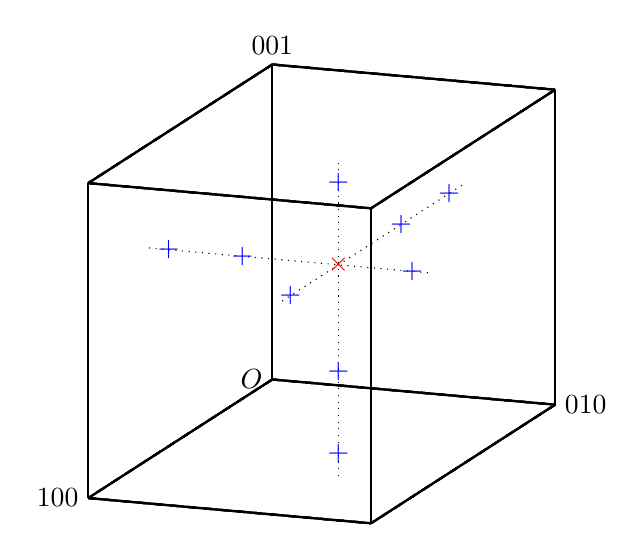
\begin{tikzpicture}[scale=4,rotate around x=270,rotate around z=258]
			% cube
			\def \c {0,1}
			\foreach \x in \c
			\foreach \y in \c
			\foreach \z in \c {
				\ifthenelse{\x = 0 \AND \y = 0 \AND \z = 0}{
					\ifthenelse{\x = 0}{\draw [dashed,thick] (0,\y,\z) -- (1,\y,\z);}{}
					\ifthenelse{\y = 0}{\draw [dashed,thick] (\x,0,\z) -- (\x,1,\z);}{}
					\ifthenelse{\z = 0}{\draw [dashed,thick] (\x,\y,0) -- (\x,\y,1);}{}
				}{
					\ifthenelse{\x = 0}{\draw [-,thick] (0,\y,\z) -- (1,\y,\z);}{}
					\ifthenelse{\y = 0}{\draw [-,thick] (\x,0,\z) -- (\x,1,\z);}{}
					\ifthenelse{\z = 0}{\draw [-,thick] (\x,\y,0) -- (\x,\y,1);}{}
				}
			}
			% annotations
			\draw (0,0,0) node[left] {$O$};
			\draw (1,0,0) node[left] {$\Node{1}{0}{0}$};
			\draw (0,1,0) node[right] {$\Node{0}{1}{0}$};
			\draw (0,0,1) node[above] {$\Node{0}{0}{1}$};
			
			% gauss legendre: 0.06943, 0.33, 0.67, 0.9306
			\def \rpg {0.67}
			\def \pgs {0.06943,0.33,0.9306}
			% pointillés
			\draw [dotted] (0,\rpg,\rpg) -- (1,\rpg,\rpg);
			\draw [dotted] (\rpg,0,\rpg) -- (\rpg,1,\rpg);
			\draw [dotted] (\rpg,\rpg,0) -- (\rpg,\rpg,1);
			% points volumiques alignés
			\foreach \x in \pgs {
				\draw (\x,\rpg,\rpg) node[blue] {$\bm{+}$};
				\draw (\rpg,\x,\rpg) node[blue] {$\bm{+}$};
				\draw (\rpg,\rpg,\x) node[blue] {$\bm{+}$};
			}
			% point volumique de référence
			\draw (\rpg,\rpg,\rpg) node[red] {$\bm{\times}$};
		\end{tikzpicture}
	\end{center}
\end{figure}


Afin de calculer le terme de rigidité \eqref{eq:terme_de_rigidite}, nous n’avons
à prendre en compte que les valeurs sur ces $3 (\Deg + 1)$ points. De plus, en chacun
de ces points, excepté $\GLN{i}$, seule la composante du gradient
correspondant à la direction d’alignement est non nulle. Cette propriété permet
encore de simplifier la programmation des calculs de ce terme
(figure \ref{img:hexa_ref_simplification}).

La matrice de rigidité est alors diagonale par bloc, chaque bloc correspondant
à une maille du maillage. Le calcul de chacun de ses termes ne nécessite que
l’évaluation de $3 (\Deg + 1)$ termes et est local à chaque maille, \textit{i.e.}
il n’y a pas d’interaction entre fonctions de base appartenant à des mailles
différentes. Cette propriété rend la parallélisation de ce terme aisée.
\\


\subsection{Terme de flux}
\label{ssect:terme_de_flux}

Le terme de « flux » permet le couplage entre les mailles voisines. Notons $\W_\L$
le champ $\W$ provenant de la maille $\L$. Le champ $\W_\R$ désignera le champ
$\W$ provenant d’une maille $\R$ ayant une face en commun (ou simplement
une surface de contact) avec la maille $\L$.
Notons également $(\QuadPhy_f)_{f \in \Range{0}{5}}$ les $6$ faces de
$\L$ image par $\TGeo{\L}$ des faces $(\QuadRef_f)_{f \in \Range{0}{5}}$
de $\HexaRef$.

Sur une face $\QuadPhy_f$ ne touchant pas le bord du domaine de calcul,
nous avons :
\begin{equation}
	\begin{aligned}
		\int_{\QuadPhy_f} &\Flux{\W_\L}{\W_\R}{\n} \PsiPhy{\L}{i} ds \\
		&= \int_{\QuadRef_f}
			\Flux{\W_\L \circ \TGeo{\L}}{\W_\R \circ \TGeo{\L}}{
				\Com{\TGeo{\L}'} \hat{\n}}
			\PsiPhy{\L}{i} \circ \TGeo{\L} d\hat{s}
	\end{aligned}
\end{equation}
où $\Com{\TGeo{\L}'}$ est la comatrice de $\TGeo{\L}'$ définie
précédemment \eqref{eq:comatrice}.


Notons $\W_{\L,f,i}$ la valeur des champs provenant de la maille $\L$
au point d'intégration $\GLNPhy{\L}{f,i}$, le $i$-ième point d'intégration de la face
$\QuadPhy_f$ de la maille $\L$. Nous avons :
\begin{align}
	\W_{\L,f,i} = \VSum{j}
	\W_{\L,j} \PsiRef{j} (\GLN{f,i}) .
\end{align}

Soit $f'$ l’indice de la face de la maille $\R$ coïncidant (ou en contact) avec la face $f$ de $\L$.
Lorsque les faces et l'ordre d'interpolation des deux mailles coïncident,
le point $\GLNPhy{\L}{f,i}$ coïncide avec un point
d'intégration de la maille $R$. Le raccord est alors dit conforme et
l'extrapolation des champs provenant de la maille voisine est
semblable à celle effectuée dans la maille $\L$.

\subsubsection{Raccord conforme}
\label{sssect:terme_de_flux_conforme}

\newcommand{\GLNFPermut}{\sigma_{\L \R}} % Permutation des points de gauss sur les faces

Soit $\GLNFPermut$, la permutation qui à l'indice $i$ du point d’intégration sur la face $f$
de $\L$ associe l'indice du point d’intégration sur la face $f'$ de $\R$ correspondant
au point $\GLNPhy{\L}{f,i}$, c’est-à-dire :
\begin{align}
	\TGeo{\R}(\GLN{f',\GLNFPermut(i)}) = \GLNPhy{\R}{f',\GLNFPermut(i)} =
	\GLNPhy{\L}{f,i} = \TGeo{\L}(\GLN{f,i}) .
\end{align}

Notons alors $\W_{\R,f',i}$ la valeur des champs provenant de la maille $\R$
au point d'intégration $\GLNPhy{\R}{f',i}$, le $i$-ième point d'intégration de la face
$\QuadPhy_{f'}$ de la maille $\R$. Nous avons :
\begin{align}
	\W_{\R,f',i} = \VSum{j}
	\W_{\R,j} \PsiRef{j} (\GLN{f',i}) .
\end{align}

Nous approchons alors l’intégrale précédente par :
\begin{equation}
	\begin{aligned}
		\int_{\QuadPhy_f} &\Flux{\W_\L}{\W_\R}{\n} \PsiPhy{\L}{i} ds \\
		&\approx \SSum{j} \GLW{f,j} \PsiRef{i}(\GLN{f,j})
			\Flux{\W_{\L,f,j}}{\W_{\R,f',\GLNFPermut(j)}}{
			\Com{\TGeo{\L}'} \hat{\n}} .
	\end{aligned}
\end{equation}

De plus, la fonction de base $\PsiRef{i}$ est non nulle en uniquement un point
d’intégration de la face $f$ (proposition \ref{prop:projection_face}).
Il s'agit du point d'intégration d'indice $j = \pi(f,i)$, projeté sur la face $f$ du point
d'intégration $\GLN{i}$ associé à la fonction de base $\PsiRef{i}$.
La somme précédente se réduit donc à un seul terme :
\begin{equation}
	\begin{aligned}
		\int_{\QuadPhy_f} &\Flux{\W_\L}{\W_\R}{\n} \PsiPhy{\L}{i} ds \\
		&\approx \GLW{f,\pi(f,i)} \PsiRef{i}(\GLN{f,\pi(f,i)})
			\Flux{\W_{\L,f,\pi(f,i)}}{\W_{\R,f',\GLNFPermut(\pi(f,i))}}{
			\Com{\TGeo{\L}'} \hat{\n}}
		\label{eq:terme_de_flux} .
	\end{aligned}
\end{equation}


Afin de calculer ce flux, nous devons calculer les champs provenant des deux
mailles voisines au point $\GLNPhy{\L}{f,\pi(f,i)}$.
L’extrapolation du champ $\W_{\L,f,\pi(f,i)}$ n’utilise que
les $\Deg + 1$ valeurs associées aux fonctions de base des points d’intégration
volumiques se projetant sur le point de face $\GLN{f,\pi(f,i)}$,
\textit{i.e.} les fonctions de base non nulles en ce point.

Lorsque les ordres d’approximation dans les deux mailles voisines sont égaux
et que les faces coïncident, le calcul de $\W_{\R,f',\GLNFPermut(\pi(f,i))}$
est semblable à celui de $\W_{\L,f,\pi(f,i)}$.


\subsubsection{Raccord non conforme}
\label{sssect:terme_de_flux_non_conforme}

Dans le cas contraire et de manière plus générale,
lorsque le point $\GLNPhy{\L}{f,\pi(f,i)}$ ne coïncide pas
avec un point d'intégration de la maille $\R$, l'extrapolation des champs provenant
de la maille voisine nécessite l'utilisation de la réciproque de la transformation
géométrique $\TGeo{\R}$ (supposée bijective).
Ce cas se présente lorsque les faces ou l'ordre d'interpolation des deux mailles ne coïncident pas.
Nous devons alors calculer le champ $\W_\R$ au point
$\TGeo{\L} (\GLN{f,\pi(f,i)})$ en appliquant la décomposition dans la base
de l'élément de référence :
\begin{align}
	\W_\R(\GLNPhy{\L}{f,\pi(f,i)}) =
	\VSum{j} \W_{\R,j}
	\PsiRef{j} \circ \Inv{\TGeo{\R}} \circ \TGeo{\L} (\GLN{f,\pi(f,i)})
	\label{eq:extract_complete} .
\end{align}

Dans cette dernière formule, l'ordre $\Deg$ de la maille $\R$ peut être différent
de celui de la maille $\L$. De plus, aucune propriété n'affirme que certains termes
de cette somme sont nuls. Il faut donc calculer les $\VNPG$ termes pour extrapoler
les champs en un point de face, contrairement au cas conforme qui ne nécessite
que le calcul de $\Deg + 1$ termes.


\subsubsection{Maille de bord}
\label{sssect:terme_de_flux_bord}


Enfin, dans le cas d’une face touchant le bord du domaine, le flux numérique est
remplacé par un flux de bord traduisant l’application d’une condition limite
spécifique. L’évaluation de ce terme de flux en un point d’intégration de cette
face nécessite comme précédemment l'extrapolation du champ de la maille $\L$ en ce point.
Afin de garantir la stabilité du schéma, le flux de bord doit satisfaire le
théorème \ref{thm:decroissance_energie} garantissant la décroissance de
l’énergie du système.

\begin{remark}
	Le calcul du terme de flux fait intervenir des champs provenant des mailles
	voisines. Ainsi, les fonctions de base appartenant à ces mailles interagissent,
	ce qui a pour effet de rendre la parallélisation du calcul de ce terme plus
	délicate et plus coûteuse en temps.
	\\
\end{remark}



\section{Schémas temporels}
\label{sect:schemas_temporels}

Après avoir donné une formulation discrétisée en espace, il est indispensable
de fournir également une technique de discrétisation en temps. Le choix du
schéma en temps est crucial. Il faut en effet s’assurer de la précision et de la
stabilité du schéma couplé espace-temps.


Nous avons décrit le calcul de la dérivée en temps du champ $\Ptl{t}\W$ en
fonction du champ $\W$ à un instant $t$ donné.
Dans cette section, nous noterons $\mathcal{G}$, l’application qui à un champ
$\W \in \mathcal{H}_h^\NC$ et un instant $t$ associe sa dérivée en temps
obtenue par la méthode GD décrite précédemment :
\begin{equation} \label{eq:operateur_gd}
	\Ptl{t}\W = \mathcal{G}(\W,t) .
\end{equation}


Soit $\dt$ un réel strictement positif de $\PbTps$. Ce réel est appelé
« pas de temps ». Notons $\W^n$ la solution numérique du problème
semi-discret \eqref{eq:formulation_semi-discrete} au temps $t_n = n \dt$. 
Supposons $\W^n$ connu pour un entier $n$ donné. Nous allons décrire comment calculer
la solution au pas de temps suivant $\W^{n+1}$.
\\

\subsection{Runge-Kutta}
\label{ssect:rk}

En pratique, nous calculons le plus souvent $\W^{n+1}$ par la méthode
de Runge-Kutta d’ordre $2$ (RK$2$) :
\begin{equation}
	\begin{aligned}
		\W^{n+\frac{1}{2}} &= \W^n
			+ \frac{\dt}{2} \mathcal{G}(\W^n,t) , \\
		\W^{n+1} &= \W^n
			+ \dt \mathcal{G}\left(\W^{n+\frac{1}{2}},t + \frac{\dt}{2}\right)
		\label{eq:methode_rk2} .
	\end{aligned}
\end{equation}
La première étape est appelée prédiction.
La seconde étape est appelée mise-à-jour.


Cependant, comme nous le préciserons dans la suite, cette méthode peut
s'avérer numériquement instable dans certains cas.
Nous avons donc aussi implémenté la méthode de Runge-Kutta d’ordre $3$ (RK$3$)
afin de bénéficier, si nécessaire, de sa condition de stabilité moins contraignante.
\\


\subsection{Condition de stabilité numérique}
\label{ssect:stabilite_numerique}

Pour étudier la stabilité du schéma GD couplé à une intégration en temps
de type RK,
nous considérons le problème d'évolution \eqref{eq:probleme_evolution} avec des
conditions aux limites impliquant l’existence et l’unicité de la solution.

Soit $\W$ la solution approchée de ce système. Notons alors $\A$ la matrice
liant la dérivée en temps $\Ptl{t}\W$ au champ $\W$. Le schéma numérique
s’écrit, en simplifiant :
\begin{align}
	\Ptl{t}\W = \A \W .
\end{align}
Dans ce cas, la solution $\W$ est donnée par :
\begin{align}
	\W(t) = \exp(\A t) \Winit .
\end{align}
Un développement de Taylor donne alors l’approximation à l'ordre $k$ :
\begin{align}
	\W^{n+1} = \tilde{\A} \W^n ,
	\; \mathrm{avec} \;
	\tilde{\A} = \sum_{i=0}^{k} \frac{(\dt)^i}{i!} \A^i
	\label{eq:developpement_taylor} .
\end{align}
Dans le cas particulier linéaire, tous les schémas d’intégration en temps d'ordre $k$ fixé
sont équivalents. Un tel schéma est stable si les valeurs propres
de la matrice $\tilde{\A}$ sont de module inférieur à $1$.
%  PH: ne pas parler de rayon spectral, dire que les vp doivent avoir un module inférieur à 1. supprimer l'inegalite de normes ci-dessus
Ces valeurs propres sont de la forme
$\sum_{i=0}^{k} \frac{(\dt \lambda)^i}{i!}$, où $\lambda$ est une valeur
propre de $\A$.
\begin{proposition} \label{prop:stabilite}
	Un schéma d’ordre $k$ est stable pour un pas de temps $\dt$ si toutes les
	valeurs propres $\lambda$ de $\A$ sont telles que $\dt \lambda$
	appartienne à :
	\begin{align}
		S_k = \left \{
			\mu \in \EnsC : \Abs{\sum_{i=0}^{k} \frac{\mu^i}{i!}} \le 1
		\right \} .
	\end{align}
\end{proposition}

On peut alors noter $C_k$ le contour de l'ensemble $S_k$, c'est-à-dire :
\begin{align}
	C_k = \left \{
		\mu \in \EnsC : \Abs{\sum_{i=0}^{k} \frac{\mu^i}{i!}} = 1
	\right \} .
\end{align}

Dans le cas du couplage GD-RK$2$, la zone de stabilité est donc donnée par l'ensemble :
\begin{align}
	S_2 = \left \{
		\mu \in \EnsC : \Abs{1 + \mu + \frac{\mu^2}{2}} \le 1
	\right \} .
\end{align}
Cet ensemble est illustré par son contour dans la figure \ref{img:zone_stabilite_rk2}.


\begin{figure}[!h]
	\begin{center}
		\caption{
			\label{img:zone_stabilite_rk2}
			Contours des zones de stabilité du schéma couplé pour les schémas temporels d'ordre $1$, $2$ et $3$.
			La zone de stabilité d'un schéma d'ordre $1$ est l'ensemble des points compris dans
			le cercle unité centré en le point d'affixe $z = -1$.
		}
		
		\begin{tikzpicture}
			\begin{axis}[
				axis lines=middle,
				xlabel=$\mathrm{Re}$, x label style={at={(axis cs:0.4,0)},anchor=north},
				ylabel=$\mathrm{Im}$, y label style={at={(axis cs:0,2.7)},anchor=east},
				xmin=-3.1,xmax=0.4,ymin=-2.7,ymax=2.7,
				xtick={-3,-2,...,0},ytick={-2,-1,...,2},
				x post scale=1.8,
				y post scale=2,
				legend style={at={(axis cs:-3,2.6)},anchor=north west}]
				\addplot[
					color=black,
					%fill=black, 
					%fill opacity=0.05
				]
				table[
					mark=none] {stab_rk1.plt};
				\addlegendentry{$C_1$ (RK$1$)}
				\addplot[
					color=red,
					%fill=red, 
					%fill opacity=0.05
					]
					table[
						mark=none] {stab_rk2.plt};
				\addlegendentry{$C_2$ (RK$2$)}
				\addplot[
					color=blue,
					%fill=blue, 
					%fill opacity=0.05
					]
					table[
						mark=none] {stab_rk3.plt};
				\addlegendentry{$C_3$ (RK$3$)}
			\end{axis}
		\end{tikzpicture}
	\end{center}
\end{figure}


Le calcul des valeurs propres de $\A$ permet donc d'assurer la stabilité
du schéma couplé en cas d'existence d'un pas de temps $\dt$ vérifiant la proposition
\ref{prop:stabilite}.
Nous constatons que dans le cas des schémas RK$1$ et RK$2$, une condition suffisante à l'existence
d'un tel pas de temps est que les valeurs propres non nulles de la matrice $\A$
aient une partie réelle négative.
%\todo{attention: zéro est en général valeur propre de A, mais ce n'est pas grave}
Le choix d'un pas de temps plus petit permet alors de
rapprocher les valeurs propres de l'axe réel jusqu'à les inclure dans la zone de stabilité.
Dans le cas du schéma RK$3$, la zone de stabilité est tangente à l'axe imaginaire
dans le demi-plan des parties réelles positives, englobant une partie de l'axe
imaginaire, ce qui permet de fortement relâcher la contrainte sur le choix du pas de temps.

Cependant, le calcul de la matrice $\A$ nécessite d'appliquer le schéma couplé
pour chaque point d'approximation du maillage, soit pour $\NE$ mailles discrétisées
à l'ordre $\Deg$, ce qui représente $6 \NE \VNPG$ degrés de liberté dans le cas
des équations de Maxwell.
De plus, pour des maillages contenant un grand nombre de mailles,
le calcul des valeurs propres de cette matrice est coûteux en temps.

Cette méthode de calcul des valeurs propres a cependant été utilisée ponctuellement
afin d'évaluer la stabilité d'une maille donnée, par exemple au cours de l'implémentation d'autres
méthodes ayant recours à des pas de temps propres à chaque maille
(méthodes dites à « pas de temps local »). Nous évoquerons
ce type de schémas dans le chapitre \ref{chap:pas de temps local}.
\\


\subsection{Condition de stabilité \emph{a priori}}
\label{ssect:stabilite_a_priori}

Devant la complexité de l'évaluation de la condition de stabilité énoncée précédemment,
nous allons présenter un critère de type CFL \cite{Courant1928},
permettant de déterminer un pas de temps
de stabilité \emph{a priori}, en fonction du maillage uniquement.

La définition d’un tel pas de temps par un critère de type CFL a fait l’objet de différents travaux,
voir par exemple \cite{kubatko2008time, Hesthaven:2007:NDG:1557392, fezoui2005convergence} pour une estimation de la stabilité du schéma
GD associé à une intégration en temps de type saute-mouton. Pour les schémas de type Runge-Kutta, il n'existe pas
encore, à notre connaissance, de résultat théorique de stabilité sur des maillages non structurés.

Nous utilisons la condition de stabilité empirique décrite par Hesthaven \textit{et al.} \cite{Hesthaven:2007:NDG:1557392} sous la forme :
\begin{align}
	\dt \le C_1 \frac{\min l_H}{v} \frac{1}{2 \Deg + 1} ,
	\label{eq:cfl1}
\end{align}
où $\min l_H$ représente la plus petite arête du maillage hexaédrique considéré, $v$ représente la vitesse de propagation dans le milieu considéré
et $C_1$ est donné par le rapport du volume d'un hexaèdre divisé par la surface
de ses faces, soit $C_1 = 1/6$.
Les valeurs propres de la matrice $\tilde{\A}$ \eqref{eq:developpement_taylor}
obtenues sur un hexaèdre quelconque sont présentés dans la figure \ref{img:zone_stabilite_rk2_vp}.
%\todo{c est la vitesse du son: changer de notation}

\begin{remark}
	Dans l'implémentation du solveur \texttt{teta-clac},
	cette condition CFL \eqref{eq:cfl1} a été implémentée avec le dénominateur
	$v (\Deg + 1)$. Les simulations d'ordre élevé exécutées avec
	cette condition plus faible se sont jusqu'alors avérées stables.
\end{remark}

Cette condition de stabilité convient parfaitement aux hexaèdres « relativement »
droits. Bien que nous n'ayons pas de critère précis pour quantifier ce degré de relativité.
Nous avons néanmoins constaté que pour certains maillages contenant des mailles très déformées,
issues du découpage de tétraèdres notamment (figure \ref{img:tetra_hexa}), il peut être nécessaire d'abaisser
le coefficient de CFL du schéma couplé GD-RK$2$.

%\todo{on parle du pas de temps local ici}
Ces instabilités liées au critère CFL sont principalement apparues au cours de résolutions
utilisant un pas de temps local (chapitre \ref{chap:pas de temps local}). En effet, lorsque le pas de temps est uniforme, il est déterminé
afin de satisfaire le critère CFL sur la plus petite maille, contrairement aux méthodes à pas de temps
local qui tiennent compte de ce critère sur chaque maille du maillage.

Les travaux de Schneider \textit{et al.} \cite{schneider2013cfl} et
Burman \textit{et al.} \cite{doi:10.1137/090757940}
donnent une formulation plus précise de la condition CFL, améliorant
la stabilité du schéma couplé GD-RK$2$ :
\begin{align}
	\dt \le C_2 \left(\frac{\min \dx}{v}\right)^{\alpha}
	\label{eq:cfl2} ,
\end{align}
où $\min \dx$ représente la plus petite distance entre deux
points d'intégration, $\alpha = 4/3$ et avec $C_2$ une constante.
Ce choix pour $\alpha$ est uniquement préconisé pour le schéma couplé
GD-RK$2$. Dans le cas d'une intégration en temps d'ordre supérieur,
nous pouvons choisir $\alpha = 1$.
%\todo{formule avec le dx**3/4 pour rk2}
%\todo{PH: et c vaut quoi ? attention: conflit de notation avec la formule cfl du dessus}


Le calcul du pas de temps à l'aide du critère \eqref{eq:cfl2} nécessite de calculer environ
$\NE (\Deg + 1)^6$ distances et est donc plus coûteux que le critère \eqref{eq:cfl2}
qui ne nécessite que le calcul d'environ $\NE 8^2$ distances.
%\todo{PH: pas vraiment important si tu ne le fais qu'une fois au début...}
Néanmoins, cette seconde formulation du critère CFL a permis une résolution stable des équations
de Maxwell avec un schéma à pas de temps local pour un cas instable avec le premier critère.
Ce qui démontre qu'elle est plus adaptée aux déformations des mailles.
\\



\begin{figure}[!h]
	\begin{center}
		\caption{
			\label{img:zone_stabilite_rk2_vp}
			Valeurs propres de la matrice $\tilde{\A}$ \eqref{eq:developpement_taylor}
			dans la zone de stabilité GD-RK$2$
			dans le cas d'un hexaèdre du cas d'application \ref{sect:tete_simplifiee}.
			La condition de stabilité utilisée est la formule \eqref{eq:cfl1}.
		}
		
		\subfloat[Valeurs propres.]{
			\label{img:zone_stabilite_rk2_vp_vp}
		\begin{tikzpicture}
		\begin{axis}[
		axis lines=middle,
		xlabel=$\mathrm{Re}$, x label style={at={(axis cs:0.02,0)},anchor=north},
		ylabel=$\mathrm{Im}$,% y label style={at={(axis cs:0,2.7)},anchor=east},
		xmin=-0.21,xmax=0.02,ymin=-0.58,ymax=0.58,
		xtick={-0.2,-0.1,0},%ytick={-2,-1,...,2},
		x post scale=1.5,
		y post scale=1.5,
		%legend style={at={(axis cs:-3,2.6)},anchor=north west}
		]
		\addplot[
		very thick,
		color=red,
		%fill=red, 
		%fill opacity=0.05
		]
		table[
		mark=none] {stab_rk2.plt};
		%\addlegendentry{$C_2$ (RK$2$)}
		
		\addplot[
		mark=x,
		only marks,
		mark options={scale=2},
		color=blue,
		]
		table {diag_vp.plt};
		\end{axis}
		\end{tikzpicture}
		}
		\\
		\subfloat[Hexaèdre.]{
			\label{img:zone_stabilite_rk2_vp_hexa}
		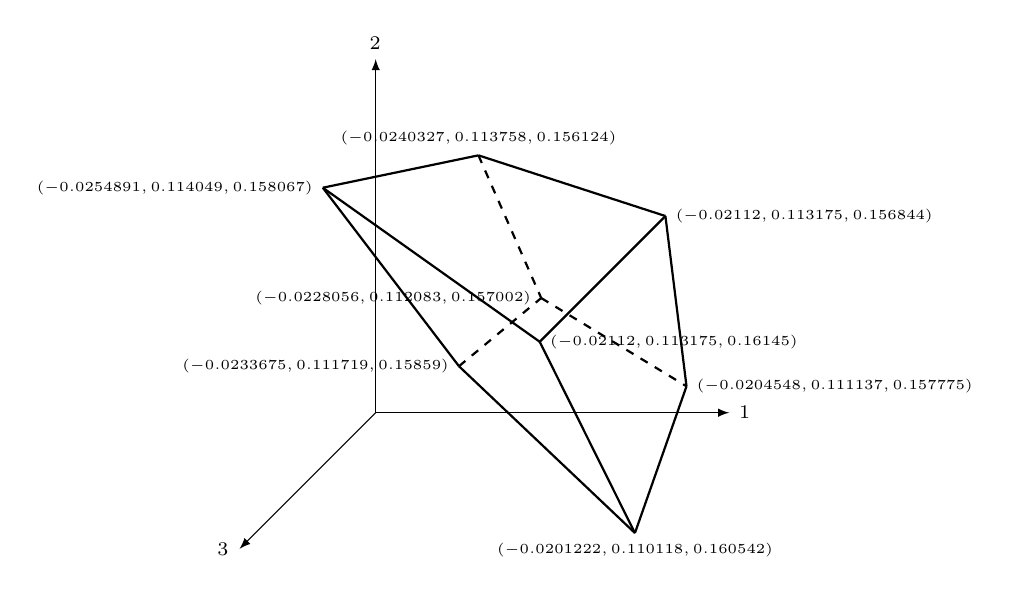
\begin{tikzpicture}[scale=900]
		\draw[arrows={-latex}] (-0.0254891, 0.110118, 0.156124) -- (-0.0204891, 0.110118, 0.156124) node[right]{$\x_1$};
		\draw[arrows={-latex}] (-0.0254891, 0.110118, 0.156124) -- (-0.0254891, 0.115118, 0.156124) node[above]{$\x_2$};
		\draw[arrows={-latex}] (-0.0254891, 0.110118, 0.156124) -- (-0.0254891, 0.110118, 0.161124) node[left]{$\x_3$};
		
		\draw[thick] (-0.02112, 0.113175, 0.16145) -- (-0.0254891, 0.114049, 0.158067)
			node[left]{\tiny$(-0.0254891, 0.114049, 0.158067)$};
		\draw[thick] (-0.0254891, 0.114049, 0.158067) -- (-0.0240327, 0.113758, 0.156124)
			node[above]{\tiny$(-0.0240327, 0.113758, 0.156124)$};
		\draw[thick] (-0.0240327, 0.113758, 0.156124) -- (-0.02112, 0.113175, 0.156844)
			node[right]{\tiny$(-0.02112, 0.113175, 0.156844)$};
		\draw[thick] (-0.02112, 0.113175, 0.156844) -- (-0.02112, 0.113175, 0.16145)
			node[right]{\tiny$(-0.02112, 0.113175, 0.16145)$};
		\draw[thick] (-0.0201222, 0.110118, 0.160542) -- (-0.0233675, 0.111719, 0.15859)
			node[left]{\tiny$(-0.0233675, 0.111719, 0.15859)$};
		\draw[thick,dashed] (-0.0233675, 0.111719, 0.15859) -- (-0.0228056, 0.112083, 0.157002)
			node[left]{\tiny$(-0.0228056, 0.112083, 0.157002)$};
		\draw[thick,dashed] (-0.0228056, 0.112083, 0.157002) -- (-0.0204548, 0.111137, 0.157775)
			node[right]{\tiny$(-0.0204548, 0.111137, 0.157775)$};
		\draw[thick] (-0.0204548, 0.111137, 0.157775) -- (-0.0201222, 0.110118, 0.160542)
			node[below]{\tiny$(-0.0201222, 0.110118, 0.160542)$};
		\draw[thick] (-0.02112, 0.113175, 0.16145) -- (-0.0201222, 0.110118, 0.160542);
		\draw[thick] (-0.0254891, 0.114049, 0.158067) -- (-0.0233675, 0.111719, 0.15859);
		\draw[thick,dashed] (-0.0240327, 0.113758, 0.156124) -- (-0.0228056, 0.112083, 0.157002);
		\draw[thick] (-0.02112, 0.113175, 0.156844) -- (-0.0204548, 0.111137, 0.157775);
		
		\end{tikzpicture}
		}
	\end{center}
\end{figure}



\subsection{Diagnostic de stabilité : Puissance itérée}
\label{ssect:puissance itérée}


Une autre technique de diagnostic des instabilités a été implémentée dans le solveur :
la méthode de puissance itérée.
\begin{proposition}
	Soit $\A$ une matrice carrée de taille $\NC$ et $(\lambda_i)_{i \in \Range{1}{\NC}}$
	ses valeurs propres telles que :
	\begin{align}
		\Abs{\lambda_1} > \max (\Abs{\lambda_2} , \dots , \Abs{\lambda_\NC}) .
	\end{align}
	Soit aussi les sous-espaces caractéristiques $(E_i)_{i \in \Range{1}{\NC}}$ de $\A$
	associés aux valeurs propres $(\lambda_i)$.\\
	Alors, si la projection de $\Winit$ sur $E_1$ n'est pas nulle, la suite de vecteurs
	$(\W^n)$ définie par la relation de récurrence :
	\begin{align}
		\forall n \in \EnsN , \W^{n+1} = \frac{1}{\Norm{\A \W^n}} \A \W^n
	\end{align}
	vérifie :
	\begin{align}
		\lim_{n \to \infty} \Norm{\A \W^n} = \Abs{\lambda_1} .
	\end{align}	
\end{proposition}

Pour appliquer cette méthode, les champs sont tout d'abord initialisés avec un bruit blanc gaussien.
Cette initialisation nous permet d'assurer (avec une très forte probabilité) que la projection
du vecteur initial sur l'espace caractéristique de la plus grande valeur propre n'est pas nulle.

\begin{figure}[!h]
	\begin{center}
		\caption{
			\label{img:app_puissance_iteree}
			Résultats d'application du diagnostic de la puissance
			itérée pour différents coefficients CFL 
			dans le cas de la simulation de la section
			\ref{sect:tete_simplifiee} à l'ordre d'interpolation spatiale $\Deg=2$.
		}
		
		\begin{tikzpicture}[scale=1]
		\begin{semilogxaxis}[
		axis lines=middle,
		xlabel=Iterations, %x label style={anchor=north},
		ylabel=$\Norm{\A \W^n}$,% y label style={at={(axis cs:0,-0.05)},anchor=east},
		xmin=1,%xmax=2500,%ymin=-0.1,
		ymax=1.002,
		%xtick={0,0.1,...,0.5},
		ytick={0.999,1,1.001},
		yticklabel style={/pgf/number format/.cd,fixed,precision=3},
		x post scale=1.5,
		y post scale=1.5,
		legend style={at={(axis cs:1000,1.002)},anchor=north west}
		]
		
		\addplot[
		thick,
		mark=none,
		color=red,
		] table {puissance_iteree/norms_cfl9.plt};
		\addlegendentry{$0.9$}
		
		\addplot[
		thick,
		mark=none,
		color=blue,
		] table {puissance_iteree/norms_cfl15.plt};
		\addlegendentry{$1.5$}
		
		\addplot[
		thick,
		mark=none,
		color=green,
		] table {puissance_iteree/norms_cfl20.plt};
		\addlegendentry{$2.0$}
		
		\addplot[
		thick,
		mark=none,
		color=orange,
		] table {puissance_iteree/norms_cfl25.plt};
		\addlegendentry{$2.5$}
		
		\addplot[
		thick,
		mark=none,
		color=purple,
		] table {puissance_iteree/norms_cfl30.plt};
		\addlegendentry{$3.0$}
		
		\addplot[
		thick,
		mark=none,
		color=pink,
		] table {puissance_iteree/norms_cfl31.plt};
		\addlegendentry{$3.1$}
		
		\addplot[
		thick,
		mark=none,
		color=red, densely dashed,
		] table {puissance_iteree/norms_cfl32.plt};
		\addlegendentry{$3.2$}
		
		\addplot[
		thick,
		mark=none,
		color=blue, densely dashed,
		] table {puissance_iteree/norms_cfl33.plt};
		\addlegendentry{$3.3$}
		

		\addplot+[
		mark=none,
		color=gray, dotted,
		] plot coordinates {
			(1,	1)
			(2500,	1)
		};
		
		\end{semilogxaxis}
		\end{tikzpicture}
	\end{center}
\end{figure}



Ensuite, à chaque étape, une normalisation globale des champs est effectuée avant d'appliquer
le schéma couplé représenté dans la proposition précédente par la matrice $\A$.
La norme des champs ainsi calculée à chaque étape tend vers le module de la plus grande valeur
propre, ce qui nous donne deux informations :
l'évolution de la norme nous indique l'état de la convergence et
la limite nous permet de nous positionner par rapport aux zones de stabilité
définies dans la proposition \ref{prop:stabilite}.

Grâce à cette méthode nous pouvons évaluer la stabilité du schéma pour
un pas de temps et un maillage donnés.
Nous avons aussi la possibilité d'affiner le calcul du pas de temps en l'augmentant jusqu'à
ce que la limite tende vers $1$.

L'inconvénient majeur de cette méthode est que la convergence est généralement
d'ordre $O(\frac{1}{n})$.
Il faut donc plusieurs milliers d'itérations afin de vérifier la stabilité du schéma.

De plus, toute source électromagnétique doit être supprimée pour l'application de ce diagnostic.
Ainsi, aucun signal ne doit être injecté, la conductivité des matériaux doit
être nulle et le modèle PML (section \ref{ssect:PML}) doit être remplacé
par le modèle de Silver-Müller (section \ref{ssect:silver_mueller}).
\\

Nous appliquons ce diagnostic sur le cas d'application étudié dans la section
\ref{sect:tete_simplifiee}. La figure \ref{img:app_puissance_iteree} présente l'évolution de la norme
$\Norm{\A \W^n}$
en fonction du nombre d'itérations pour différents coefficients CFL.
Le diagnostic a été mené jusqu'à
$10$k itérations dans les cas stables, bien que nous ne présentons
que les $1000$ premières.
Nous constatons que cette simulation est stable pour un coefficient CFL
de $3.1$ et instable au-delà, pour une interpolation spatiale d'ordre $\Deg=2$.
%Nous ne dépasserons cepandant pas le coefficient CFL $1.4$
%dans la section \ref{sect:tete_simplifiee}.
Pour l'ordre spatial $\Deg=1$, le coefficient CFL de stabilité maximal
ainsi déterminé est de $4.5$.


\begin{remark}
	En temps normal, un coefficient CFL ne doit pas dépasser $1$. Cette assertion
	est vraie lorsque la condition CFL est exacte. Or, la condition
	\eqref{eq:cfl1} est empirique et fonctionne dans la plupart des cas,
	mais sans être exacte. Il arrive donc que certaines simulations soient
	instables avec un coefficient CFL de $0.9$.
	Il arrive aussi, comme dans le cas ci-dessus, qu'une simulation soit
	stable avec un coefficient CFL supérieur à $1$.
\end{remark}






\section*{Conclusion}



Dans ce chapitre, nous avons introduit l'espace d’approximation
dans lequel nous chercherons la solution numérique de notre problème.
Cet espace est représenté par un élément de référence : le cube unité, 
et muni de fonctions de base qui vont nous permettre d'exprimer
la solution à l'aide de coordonnées discrètes.
Ces fonctions de base sont les produits tensoriels des polynômes de Lagrange
qui s'appuient sur les points de Gauss-Legendre dans chaque direction.
Une transformation géométrique nous permet alors de passer
de l'élément de référence à n'importe quelle maille physique.
Nous sommes donc en mesure de résoudre tout type de problème
d'électromagnétisme modélisé à partir de mailles hexaédriques.

Cet espace d'approximation a été choisi pour ses propriétés de
simplification des formules de quadrature par l'annulation
du gradient des fonctions de base en de nombreux points d'interpolation.
Ces simplifications n'apparaissent pas dans les mailles tétraédriques.

Nous avons ensuite présenté les schémas de type Runge-Kutta
qui vont nous permettre d'intégrer temporellement la solution
afin d'avancer cette dernière jusqu'au temps final souhaité.
L'implémentation de ces schémas ne présente pas de difficulté.
Cependant, leurs conditions de stabilité sont très contraignantes.
Nous verrons un autre type de schéma, permettant de réduire
l'impact de ces contraintes, dans le chapitre \ref{chap:pas de temps local}.
\\


Dans le chapitre suivant,
nous décrivons l’implémentation sur un ou plusieurs
accélérateurs, comme des GPU ou des CPU multicœurs, de la méthode GD sur hexaèdres.
Les cartes graphiques sont toujours plus utilisées dans la simulation numérique
et permettent de paralléliser le traitement de grandes quantités de données.
Dans le cas de notre solveur, les simplifications induites par les hexaèdres
permettent la parallélisation efficace du code.

